

\chapter{Single dimension model combination\label{sec:combination}}

All models are designed for $352 \times 352$ crops of the 2D slices.
The estimation of the slice is obtained by combining the model estimations on all crops taken from this slice.

\section{Volume combination procedure}

Combining the results of three different single dimension models is performed in two steps:
\begin{enumerate}
    \item The resulting classification volumes are first combined with a rule-based method
    \item After this rule-based combination, the resulting segmentation estimation is smoothened with a morphological filter.
\end{enumerate}

\subsection{Rule based result combination}
Three single dimension models are trained:
\begin{description}
    \item[Transverse slices] offer little context to indicate which of the lumbar vertebrae they contain. 
    It does not seem easy even for a human expert to indicate which vertebra is visible on the slice.
    The model trained on these slices is intended only for semantic segmentation.
    Each pixel is inferred only if it represents a vertebra, without distinction between the different lumbar vertebrae. 
    \item[Sagittal \& Coronal slices] do offer the necessary context to distinguish between $L_1$ to $L_5$. 
    The models trained on these slices do indicate the specific lumbar vertebra index. 
\end{description}

Based on the observation that all trained models accurately predict the background, these three models are combined in a straightforward way\footnote{
    The resulting estimations from a model for an input volume is again a three-dimensional volume ($\in \mathbb{N}^3$) with the same dimensions.
}.

\begin{algorithm}[H]
    \SetAlgoLined
    \KwData{
        Results $y_.$ of three models indicating an estimated class for all positions $\vec{p}$ in the volume.
        \begin{itemize} 
            \item Transverse model $y_t \in \mathbb{N}^3: \forall y_t(\vec{p}) \in \{ 0, 1 \}$
            \item Sagittal model $y_s \in \mathbb{N}^3: \forall y_t(\vec{p}) \in \{ 0, 1, 2, 3, 4, 5 \}$ 
            \item Coronal model $y_c \in \mathbb{N}^3: \forall y_t(\vec{p}) \in \{ 0, 1, 2, 3, 4, 5 \}$ 
        \end{itemize}
    }
    \KwResult{Combination of the three model results $y_f$.}
    \For{all $\vec{p}$}{
        \eIf{$y_t[\vec{p}] = 1 \wedge y_s[\vec{p}] = y_c[\vec{p}]$}{
            $y_f[\vec{p}] \leftarrow y_s[\vec{p}]$ \;
        }{
            $y_f[\vec{p}] \leftarrow 0$ \;
        }
    }
   \caption{Rule based combination of model results from three single dimension models}
\end{algorithm}

\todo[inline]{Image illustrating the combination}

\subsection{Morphological smoothing}
After the rule-based combination of estimations from different single dimension models, the result is smoothened with standard morphological filters.
These filters are combinations of the morphological \textit{erosion} and \textit{dilation} operators.
\todo[inline]{How deep should these morphological filters be discussed?}
\begin{itemize}
    \item Possible noise is suppressed by first opening and then closing the volumes.
    \item The estimated volumes are observed to overestimate the extent of the vertebrae. For this reason, an erosion step is performed to decrease the overall extent of the class masks.
\end{itemize}

The procedure mentioned above has two Hyperparameters: the number of iterations for the denoising filters and the number of iterations for the erosion filter.
Both hyperparameters are estimated by calculating the same evaluation metric, the weigh dice score on the validation set, as for the single-dimensional model evaluation. 


\begin{SCfigure}[][htb]
    \centering
    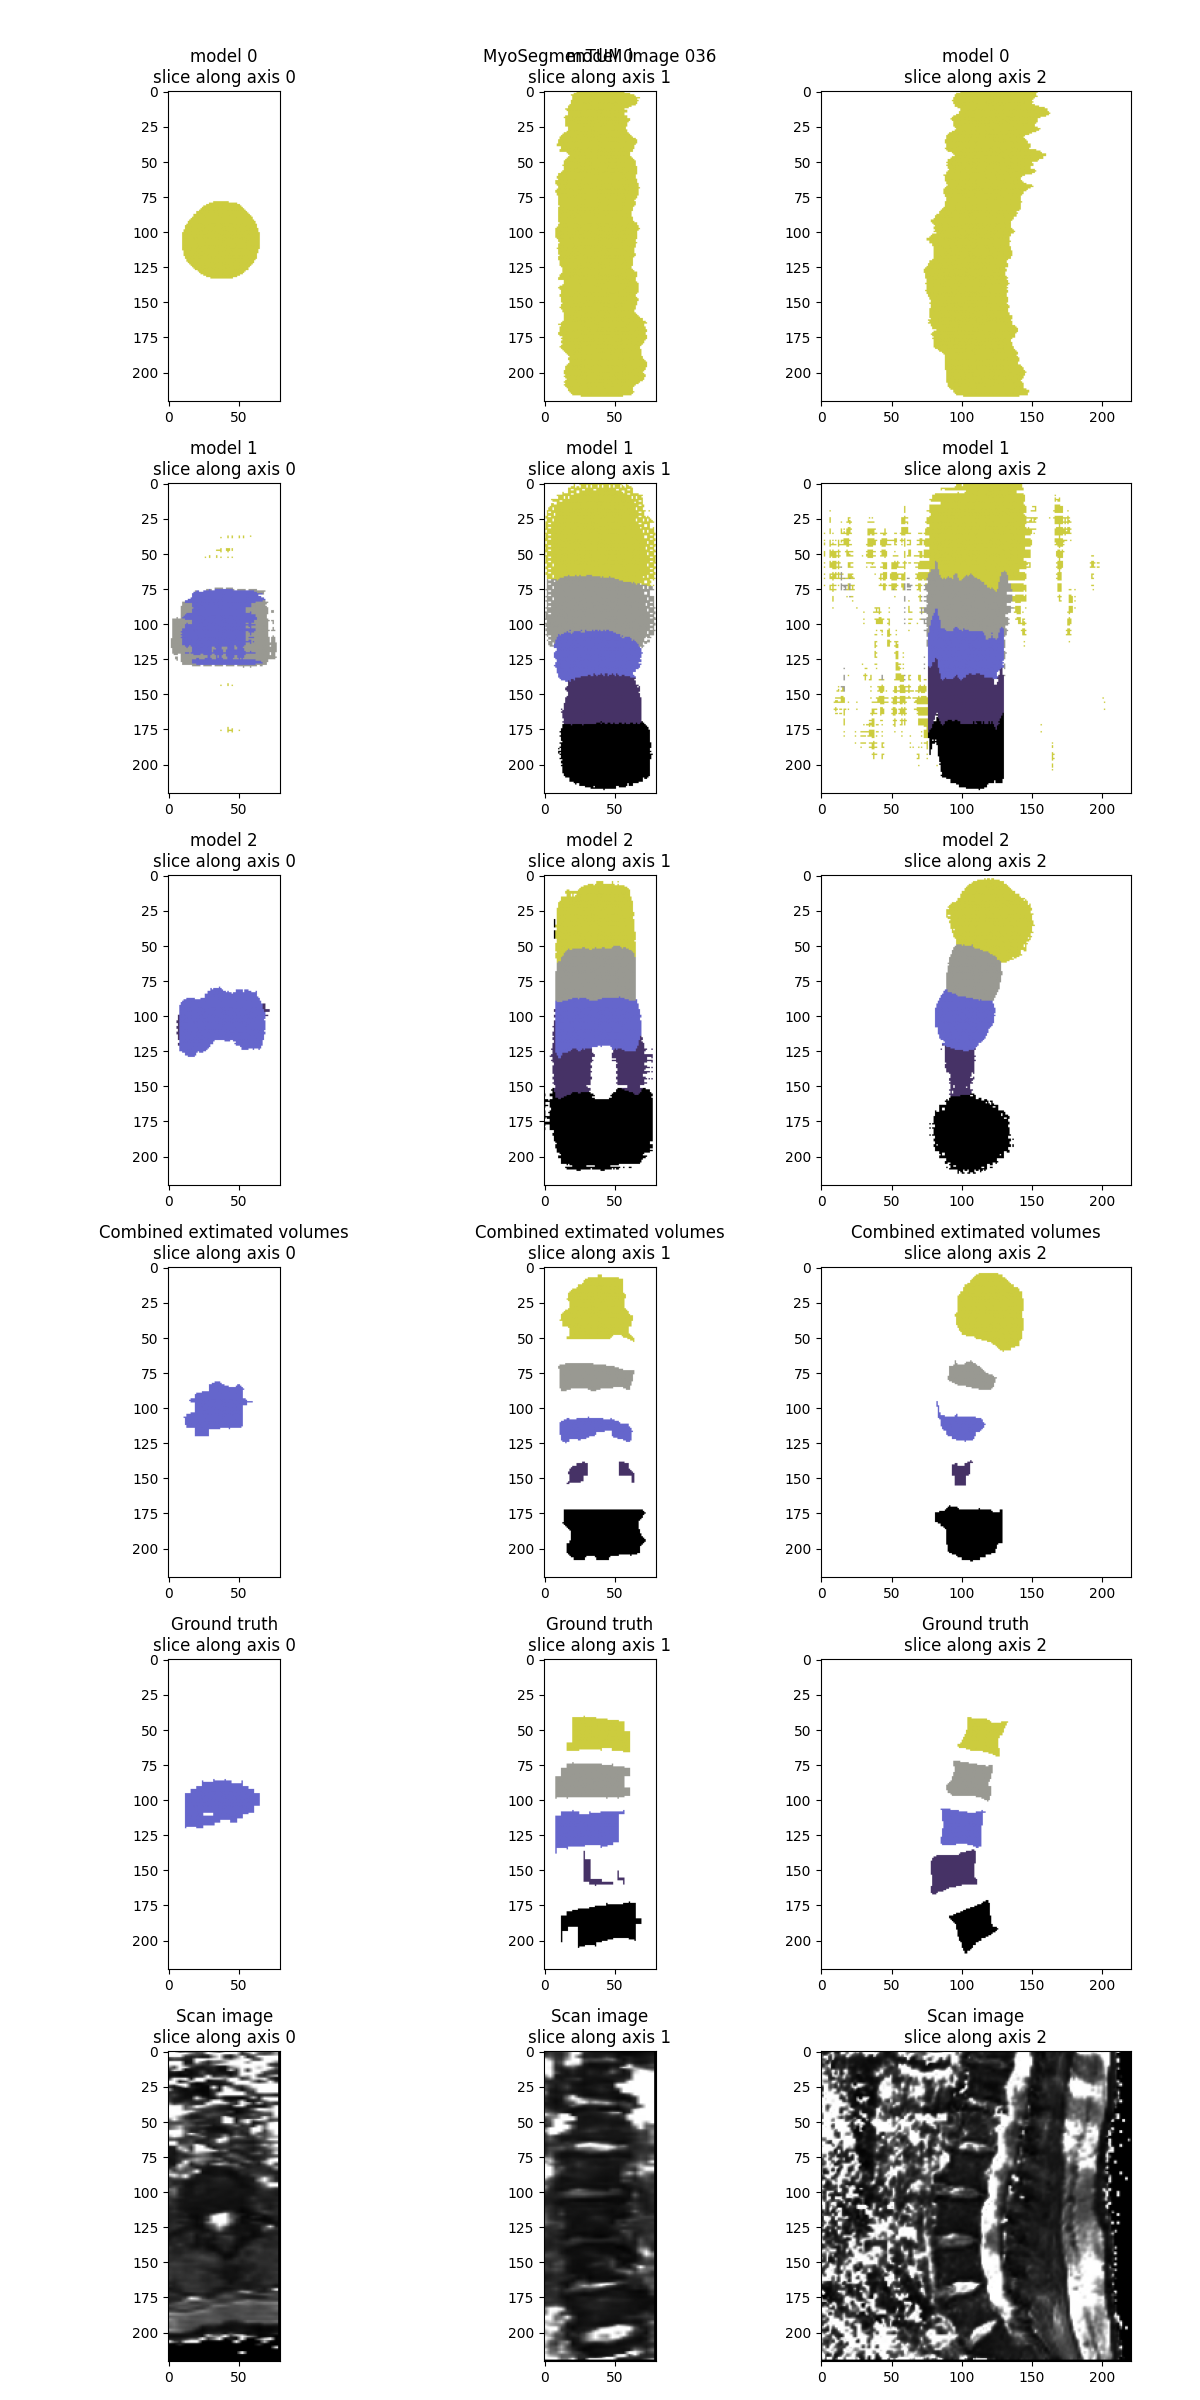
\includegraphics[width=.95\textwidth]{images/morphmask_denoise1_erode1_MyoSegmenTUM_036.png}
    \caption{
        Result of the combination of the three single dimension model results for volume MyoSegmenTUM nr 43.
        The colours indicate the vertebra classes. Only one semantic class is estimated in the first row, illustrating the model trained on transversal slices.
        On the first three rows, slices of the resulting segmentations from the single dimension models are shown. 
        It is clear these masks contain some artefacts and are not always in agreement with each other.
        On the fourth row, the result after mask combination and morphological smoothing is shown. 
        This corresponds more closely to the ground truth mask, shown on the fifth row.
        This final mask, shown on the fourth row, will be used as a pseudo mask to approximate the unknown ground truth mask.
        In the last row, the corresponding images are shown.
    }
\end{SCfigure}

\section{Pseudo mask performance}

\chapter{Pseudo mask training}
